\documentclass[letterpaper,11pt]{scrreprt}
\usepackage[american]{babel}
\usepackage[latin1]{inputenc}
\usepackage[T1]{fontenc}
\usepackage[top=1in,bottom=1in,left=1in,right=1in]{geometry}
\usepackage{lmodern}

\usepackage{amsmath}
\usepackage{amssymb}

\usepackage[amsmath,hyperref,thmmarks]{ntheorem}
\usepackage[
	bookmarks,
	colorlinks=false,
	linkcolor=blue,
	citecolor=blue,
	pagebackref=false,
	pdftitle={CloudKeeper Design Document},
	pdfauthor={SVBio},
	pdfsubject={},
	pdfkeywords={}
]{hyperref}
\usepackage{csquotes}                  % Strongly recommended for biblatex
\usepackage[
	backend=bibtex,
	maxnames=2,
	maxbibnames=20,
	firstinits=true
]{biblatex}
\usepackage{scrpage2}                  % Headers and footers
\usepackage{color}                     % Colors, possibly only for \todo
\usepackage{enumitem}                  % enumerate environment
\usepackage{subcaption}
\usepackage{ctable}
\usepackage{tabularx}
\usepackage{xspace}                    % Correct spaces after \newcommand definitions
\usepackage[noend]{algpseudocode}      % algorithm environment
\usepackage{listings}                  % Code snippets
\usepackage{bbding}
\usepackage{latex/tikz-uml}            % UML diagrams

% BEGIN Doc Layout
	\allowdisplaybreaks[3]

	\pagestyle{scrheadings}
	\automark[chapter]{section}

	\setkomafont{disposition}{\normalcolor\bfseries}
	\setkomafont{descriptionlabel}{\bfseries}
	\setkomafont{captionlabel}{\usekomafont{disposition}}

	\setlength{\arrayrulewidth}{.5pt}
	\numberwithin{equation}{section}
	\renewcommand{\theenumi}{\roman{enumi}}
	\renewcommand{\labelenumi}{\theenumi)}

	\newcommand{\otoprule}{\midrule[\heavyrulewidth]}

	\setcounter{secnumdepth}{3}

	\makeatletter
	% Algorithms are expected to have an optional argument of form
	% FunctionName$(ArgumentList)$, e.g., DiscreteSample$(A, w)$
	\def\internal@funcName#1$(#2)${#1}
	\newcommand\funcName[1]{\internal@funcName #1}
	\newtheoremstyle{algorithm}
		{\item[\rlap{\vbox{\hbox{\hskip\labelsep \theorem@headerfont
			##1\ ##2\theorem@separator}\hbox{\strut}}}]}%
		{\item[\rlap{\vbox{\hbox{\hskip\labelsep {\theorem@headerfont
			##1}\ \normalfont\texttt{##3}{\theorem@headerfont\theorem@separator}}\hbox{\strut}}}]%
			\def\@currentlabel{\texttt{\funcName{##3}}}}
	\makeatother

	\makeatletter
	% Also display JSTOR in small caps
	% http://sourceforge.net/tracker/index.php?func=detail&aid=3152938&group_id=244752&atid=1126006
	\DeclareFieldFormat{eprint:arxiv}{%
	  \textsc{arXiv}\addcolon
	  \ifhyperref
	    {\href{http://arxiv.org/\abx@arxivpath/#1}{%
	       \nolinkurl{#1}%
	       \iffieldundef{eprintclass}
		 {}
		 {\addspace\texttt{\mkbibbrackets{\thefield{eprintclass}}}}}}
	    {\nolinkurl{#1}
	     \iffieldundef{eprintclass}
	       {}
	       {\addspace\texttt{\mkbibbrackets{\thefield{eprintclass}}}}}}
	\DeclareFieldFormat{eprint:jstor}{%
	  \mkbibacro{JSTOR}\addcolon\space
	  \ifhyperref
	    {\href{http://www.jstor.org/stable/#1}{\nolinkurl{#1}}}
	    {\nolinkurl{#1}}}
	% Some conferences do not have DOIs for their papers, but they do get
	% IDs in the ACM Digital Library. E.g., SODA papers.
	\DeclareFieldFormat{eprint:acm}{%
	  \mkbibacro{ACM}\addcolon\space
	  \ifhyperref
	    {\href{http://dl.acm.org/citation.cfm?id=#1}{\nolinkurl{#1}}}
	    {\nolinkurl{#1}}}
	\makeatother
	
	\newlist{moduleinfo}{description}{2}
	\setlist[moduleinfo]{style=multiline,labelindent=\leftmargini,leftmargin=3cm,rightmargin=\leftmargini,font=\bfseries}
	\newlist{modulehistory}{description}{2}
	\setlist[modulehistory]{style=multiline,leftmargin=1.1cm}
% END Doc Layout

% BEGIN General Definitions
	\newcommand{\todo}[1]{\textbf{\color{red}#1}}

	\newcommand{\specialcell}[3][t]{%
		\begin{tabular}[#1]{@{}#2@{}}#3\end{tabular}}

	% BEGIN Mathematical Definition
		% Space (only) in displaymath (e.g., between mathematical expression and punctuation mark)
		\newcommand{\SiM}{\mathchoice{\,}{}{}{}}
	% END Mathematical Operators

	% BEGIN URLs
		\newcommand{\mailto}[1]{\href{mailto:#1}{\nolinkurl{#1}}}
		\newcommand{\doi}[1]{DOI: \href{http://dx.doi.org/#1}{\nolinkurl{#1}}}
	% END URLs

	\makeatletter
	% BEGIN Mathematical Definitions
		% BEGIN Set Symbols
			\newcommand{\setsymbol}[1]{\mathbb{#1}}
			\newcommand{\N}{\@ifstar{\setsymbol{N}_0}{\setsymbol{N}}}
			\newcommand{\R}{\setsymbol{R}}
		    \newcommand{\Nupto}{\@ifstar{\Nupto@star}{\Nupto@nostar}}
		    \newcommand{\Nupto@star}[1]{[#1]_0}
		    \newcommand{\Nupto@nostar}[1]{[#1]}
		% END Set Symbols
		\renewcommand{\vec}[1]{\ensuremath{\boldsymbol{#1}}}
		\newcommand{\pow}[1]{2^{#1}}
	% END Mathematical Definitions
	\makeatother

	\renewcommand{\vec}[1]{\ensuremath{\boldsymbol{#1}}}
	\newcommand{\enumref}[1]{(\ref{#1})}

	\makeatletter
	\newcommand{\symlabel}[2]{\def\@currentlabel{\texttt{#1}}\texttt{#1}\label{#2}}
	\makeatother
	
	\newcommand{\Warning}[1]{\marginpar[\HandRight]{\HandLeft}\textbf{#1}}

	% BEGIN Algorithms
	\theoremstyle{algorithm}
	\theorembodyfont{\upshape}
	\newtheorem{algorithm}{Algorithm}[section]

	\newlength{\alglabelwidth}
	\newcommand{\alginput}[1]{%
		\par\noindent%
		\settowidth{\alglabelwidth}{\emph{Require:}}%
		\makebox[\alglabelwidth][l]{\emph{Input:}} \begin{tabular}[t]{l} #1 \end{tabular}}
	\newcommand{\algoutput}[1]{%
		\par\noindent%
		\settowidth{\alglabelwidth}{\emph{Require:}}%
		\makebox[\alglabelwidth][l]{\emph{Output:}} \begin{tabular}[t]{l} #1 \end{tabular}}
	\newcommand{\algprecond}[1]{%
		\par\noindent%
		\settowidth{\alglabelwidth}{\emph{Require:}}%
		\makebox[\alglabelwidth][l]{\emph{Require:}} \begin{tabular}[t]{l} #1 \end{tabular}}
	\algnewcommand{\LineComment}[1]{\State $\triangleright$ #1}

	\newcommand{\set}{\leftarrow}
	\DeclareMathOperator{\random}{random}
	\newcommand{\dist}{\ensuremath{\mathit{dist}}}
	\newcommand{\List}{\mathrm{List}}
	\newcommand{\Sample}{\mathit{Sample}}
	\algblockdefx[With]{With}{EndWith}%
		[1]{\textbf{with} #1 \textbf{do}}%
		[0]{End}
	\algnotext[With]{EndWith}
	% END Algorithms

	% BEGIN Theorem environments
		\theoremstyle{plain}
		\theoremseparator{.}

		\theoremheaderfont{\itshape}
		\newtheorem{claim}[equation]{Claim}

		\theoremheaderfont{\normalfont\bfseries}
		\theorembodyfont{\itshape}
		\newtheorem{theorem}[equation]{Theorem}
		\newtheorem{lemma}[equation]{Lemma}
		\newtheorem{corollary}[equation]{Corollary}

		\theorembodyfont{\normalfont}
		\theoremsymbol{$\lozenge$}
		\newtheorem{definition}[equation]{Definition}
		\newtheorem{example}[equation]{Example}
		
		\theoremstyle{nonumberplain}
		\theoremheaderfont{\itshape}
		\theoremsymbol{$\square$}
		\newtheorem{proof}{Proof}
		
		\theoremsymbol{$\blacksquare$}
		\newtheorem{subproof}{Proof}
	% END Theorem environments


	% BEGIN lstlisting environments
	\lstset{
		basicstyle=\ttfamily\footnotesize,       % the size of the fonts that are used for the code
		numbers=left,                   % where to put the line-numbers
		numberblanklines=false
		numbersep=1em,                  % how far the line-numbers are from the code
		basewidth=0.52em,
		tabsize=4,  		% sets default tabsize to 2 spaces
		xleftmargin=\leftmargini
	}
	\renewcommand*\thelstnumber{\the\value{lstnumber}:}
	% END lstlisting environments
	
	\lstnewenvironment{sql}[1][]{\lstset{language=SQL,gobble=4,emphstyle=\textit,#1}}{}
	\lstnewenvironment{cpp}[1][]{\lstset{language=C++,gobble=4,emphstyle=\textit,#1}}{}
	\lstnewenvironment{cppsnippet}[1][]{\lstset{basicstyle=\ttfamily,language=C++,stepnumber=0,gobble=8,emphstyle=\textit,xleftmargin=0pt,#1}}{}
% END General Definitions

\bibliography{../literature.bib}

\graphicspath{{chapters/}}

% BEGIN Preamble
\title{%
	CloudKeeper Design Document%
}

\begin{document}

\maketitle

\tableofcontents

% When using TeXShop on the Mac, let it know the root document. The following must be one of the first 20 lines.
% !TEX root = ../design.tex

\chapter{Requirements}

% Abstract.


\section{Goals}

Data-analysis tasks typically involve many different processing steps such as cleansing, loading, model training, scoring, etc. This is particularly true in bioinformatics, where processing steps often call closed-source software components or even external third-party entities (e.g., an external company that sequences blood samples). In the past, different processing steps and different tools have often been chained together by simple ad-hoc scripts written in general-purpose languages like bash, Python, or Perl. While this provides lots of freedom, these script languages are ill-suited for chaining data manipulation steps together. Indeed, this approach of defining workflow suffers from unneeded verbosity---making it hard to see the forest for the trees. Specifically:

\begin{itemize}
	\item Domain experts responsible for setting up workflows are not usually experts in programming. They wish to use convention-over-configuration or best-practices-over-do-it-yourself ways to define workflows.
	\item The burden of providing modularity and reusability is placed entirely on people who implement these scripts. Consequently, reinventions of the wheel are frequent.
	\item Most script languages are imperative languages that encourage a sequential way of thinking, which makes it hard to parallelize or distribute workflows over multiple machines or locations.
\end{itemize}

The goal of CloudKeeper is to solve the above issues, i.e., to provide a high-level interface for defining workflows. Most generally, workflows are directed graphs, where nodes represent processing steps and edges represent data flow. As such, workflows can be defined entirely by drawing connections within a graphical user interface. (More advanced users may still prefer a simple domain-specific language for defining the workflow graph.) ``Programming'' in terms of data flow transfers responsibility for ordering the processing steps to the runtime environment, i.e., the CloudKeeper core. Therefore, distributing the different processing steps efficiently across multiple machines is immediately available to all workflows and requires no user intervention.

While dataflow programming has existed since the 1960's, none of the available workflow engines satisfy all of our needs.
% When using TeXShop on the Mac, let it know the root document. The following must be one of the first 20 lines.
% !TEX root = ../design.tex

\chapter{Workflows}

% Abstract. What is the problem we want to solve?
A workflow is a directed graph, where nodes represent processing steps and edges represent data flow. A processing step can only execute when all data from incoming edges is available. It then performs its processing, and the output is eventually provided over the outgoing edges. Workflow is a recursive concept in that a node may contain another (nested) workflow. Special nodes are provided for modeling control flow (loops, branches).

\section{Requirements}

\subsection{Non-functional}

\begin{enumerate}
	\item \label{enum:NFR:W1} Usability: Developing a workflow out of existing modules should be easy and not require programming skills
	\item \label{enum:NFR:W2} Security: Developing/editing workflows must not introduce security risks (like arbitrary code execution)
	\item \label{enum:NFR:W3} Extensibility: Workflows should be expressive enough for anticipated future needs. 
	\item \label{enum:NFR:W4} Scalability: Workflows should allow compact representations that fit into the memory of individual machines. Whenever possible, workflows should facilitate parallel processing.
	\item \label{enum:NFR:W5} Maintainability: Workflows should be modular for easy reuse.
\end{enumerate}

\subsection{Functional}

\begin{itemize}
	\item Multiple in-/out ports per module
	
		Reason: Obvious

	\item Workflows must be specifiable in a simple domain-specific language

		Reason: NFR \ref{enum:NFR:W1}, \ref{enum:NFR:W2}: Only alternative is creating workflows programmatically, a clear violation of the NFRs.

	\item Workflows must have intuitive graphical representations (and eventually facilitate GUI tools)
		
		Reason: NFR \ref{enum:NFR:W1}

	\item Control flow

		Reason: NFR \ref{enum:NFR:W3}, \ref{enum:NFR:W4}: Do not force developers to hide control flow in modules, which the scheduler could then only treat as black boxes.
		\begin{itemize}
			\item Data parallel execution (either due to parallelizable loop or parallel graph) 

				NFR \ref{enum:NFR:W4}
			\item Loops with dynamic exit conditions

				NFR \ref{enum:NFR:W3}. This is needed for any iterative algorithm.
			\item Conditional execution paths

				NFR \ref{enum:NFR:W3}.
		\end{itemize}
	\item Workflows must be embeddable in other workflows, and thus be recursive structures
		
		Reason: NFR \ref{enum:NFR:W5}
\end{itemize}

\section{Workflows and Modules}

A workflow is a directed acyclic graph where nodes represent modules, and edges represent data dependencies between modules. Workflows and modules are recursive concepts in that a module may contain a sub-workflow (i.e., a subgraph). A module defined as a workflow is called \emph{composite module}, a non-composite module is called a \emph{simple module}.

Each module contains a list of ports through which data flows. The computational model for a module is simple: It takes its input through its in-ports, performs processing, and then returns output through its out-ports. When modeled as a graph, each node is hence labeled with a list of input and a list of output ports. Each edge is labeled with a source port (which must be one of the source node's output ports) and a destination port (one of the destination node's input ports).

For composite modules that contain nested modules, additional rules apply that allows linking between the two nesting levels: An in-port of a composite module may also serve as an out-port for connections to the nodes within the composite module's subgraph. Likewise, the out-ports of a composite module may be in-ports for edges from its subgraph's nodes. Edges between different subgraphs are otherwise not allowed. Moreover, an edge may only connect ports that are \emph{type-compatible}, as described in Section~\ref{sec:TypeSystem}.

\begin{example}
Before describing the different modules in detail, it is helpful to look at an example, as shown in Figure~\ref{fig:WorkflowExample}. It shows how logistic regression could be implemented as a CloudKeeper workflow. The informal description is: Take a file with data points, split this files into manageable chunks, then compute matrix $A := X^T D X$ and vector $\vec b := X^T D \vec z$ for each file separately ($X$ is the design matrix corresponding to only that file, and $D$ and $z$ are transformations of $X$ and $\vec \beta$), sum up all $A$'s and $\vec b$'s over all files, compute $\vec \beta := A^{-1} \cdot \vec b$, and iterate until the log-likelihood of $\vec \beta$ has converged.

Note that Figure~\ref{fig:WorkflowExample} is a CloudKeeper-generated GraphViz visualization of a real workflow that should be read as follows: A rectangle represents a module, which is labeled with its instance name (first line) and its module name (second line). Grey rounded boxes represent in-ports of the module, and black rounded boxes represent out-ports. A rounded box with a dotted outline represents a special port like the continue-port of a loop module.
\end{example}

\begin{figure}
	\centering
	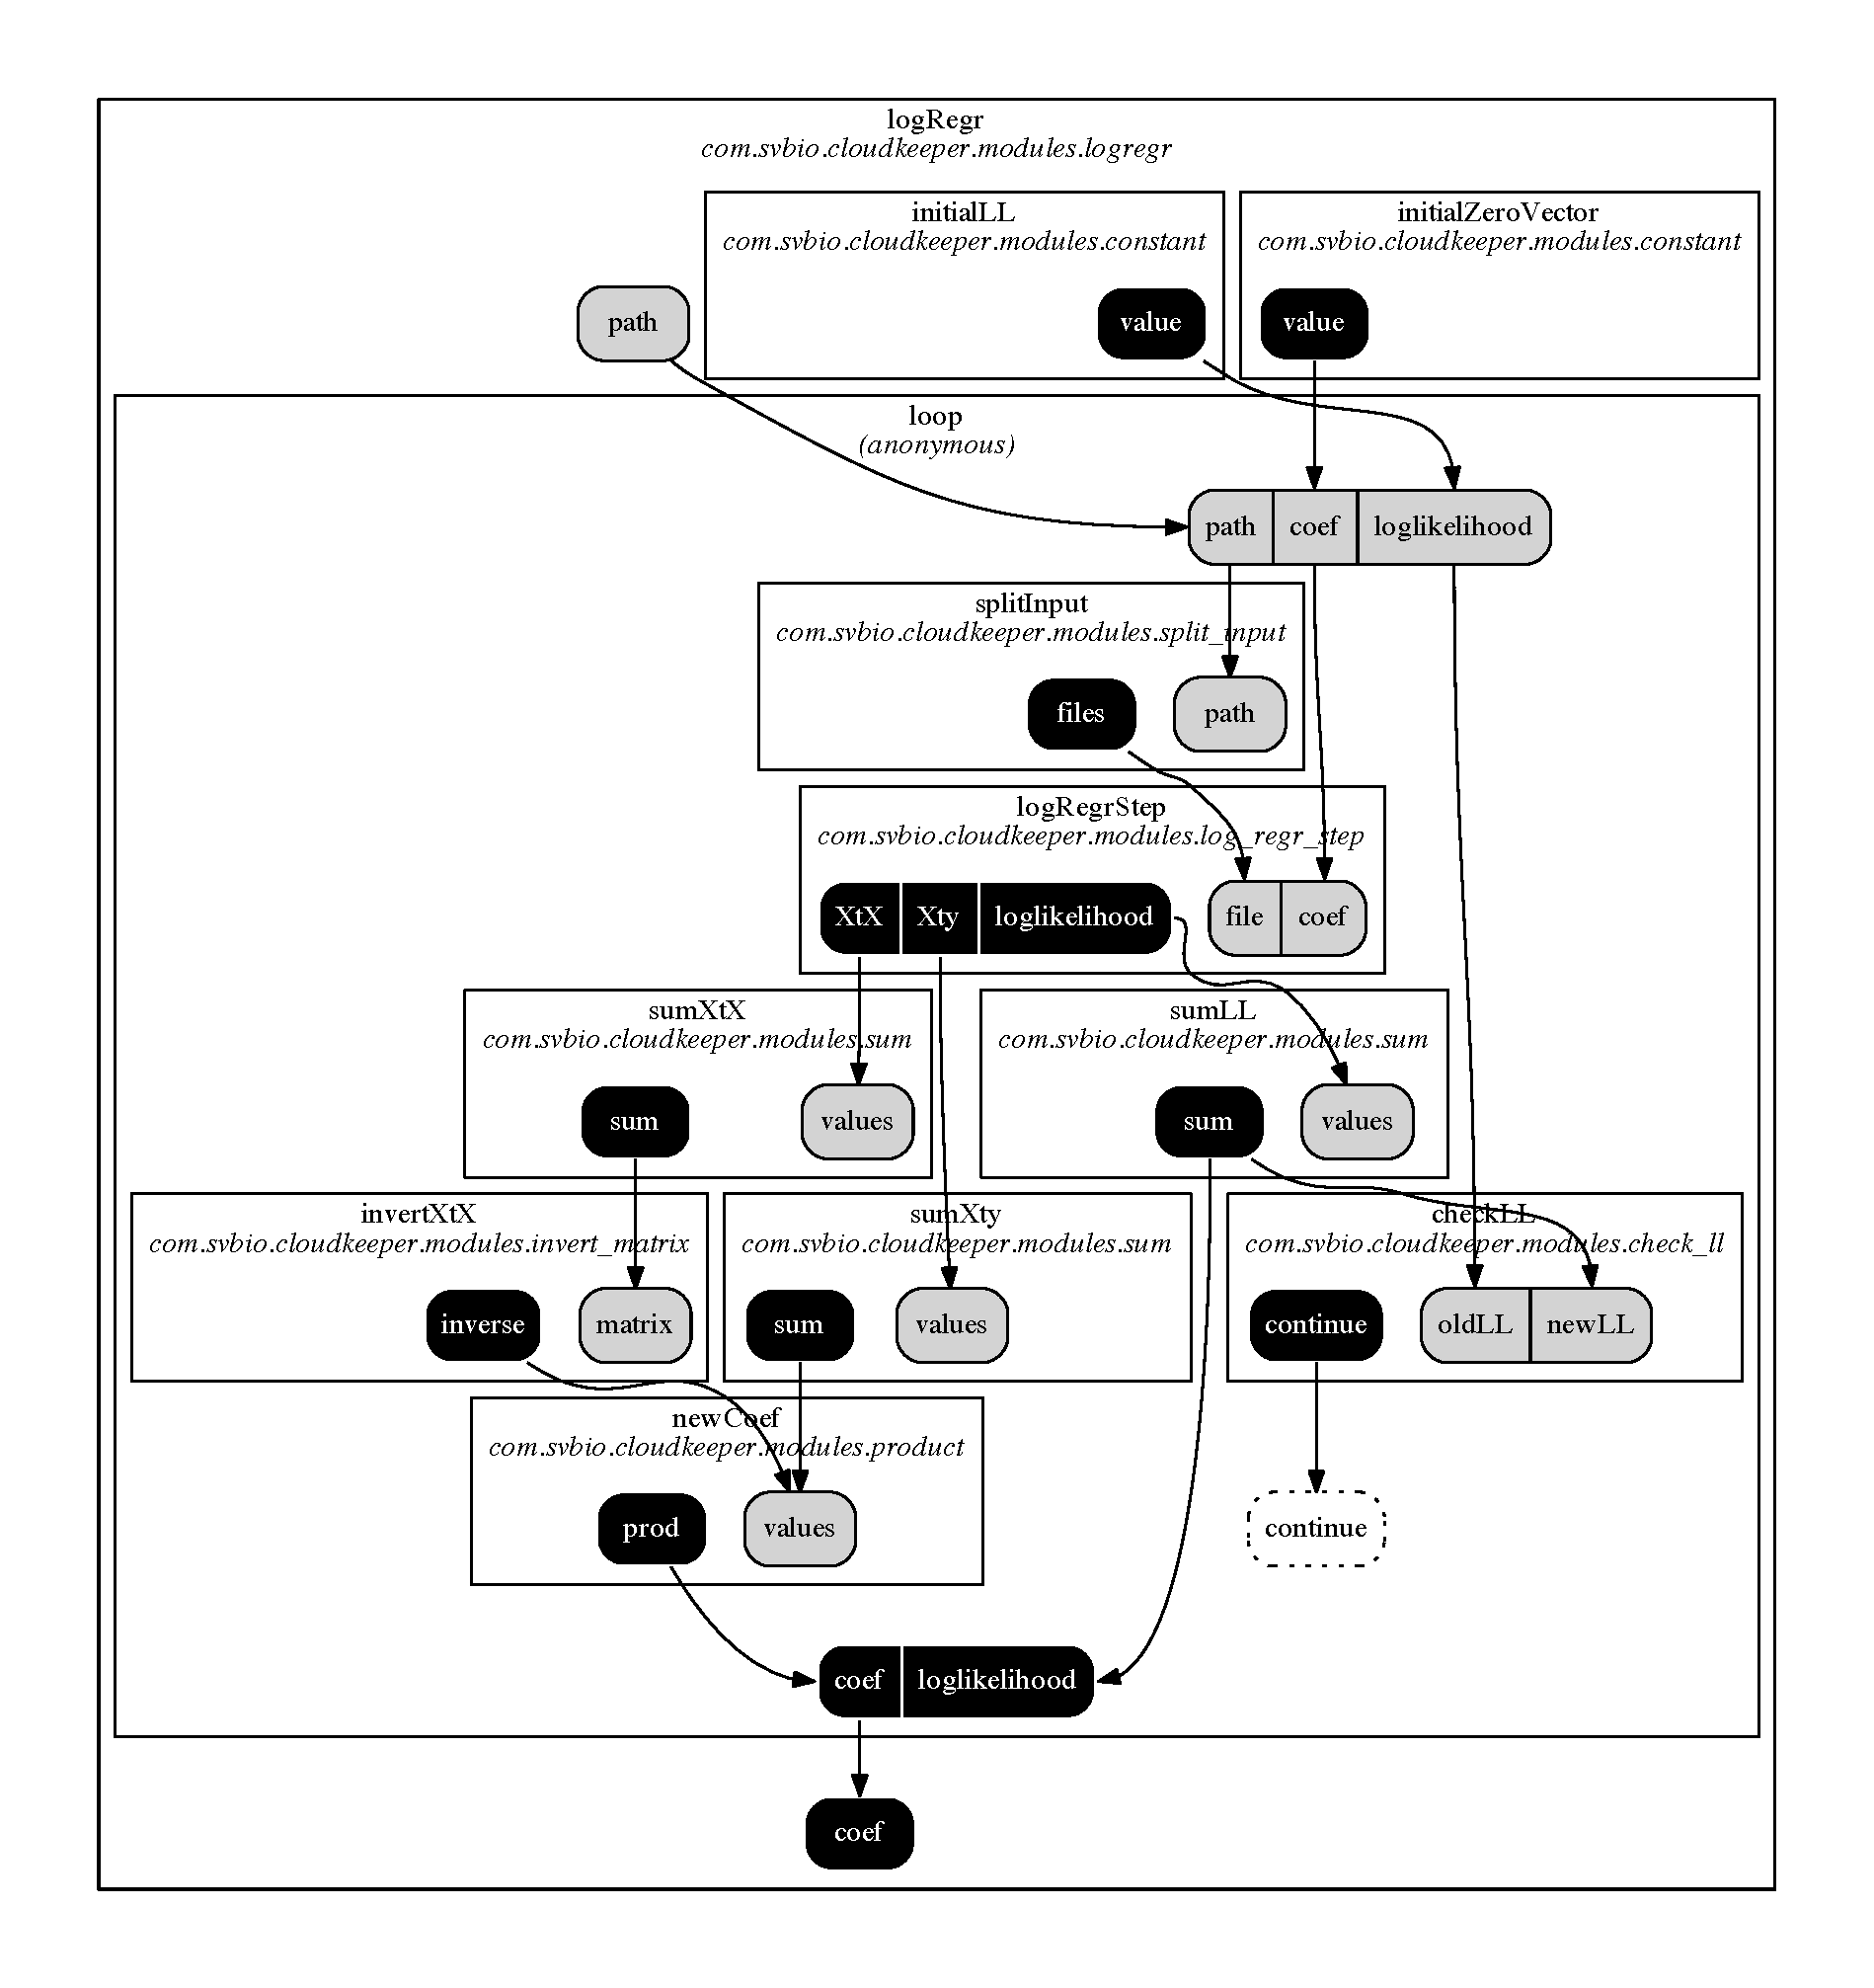
\includegraphics[width=\textwidth]{workflows/workflow-example}
	\caption{Example Workflow: Iteratively Reweighted Least Squares to Perform a Logistic Regression\label{fig:WorkflowExample}}
\end{figure}

\subsection{Module Hierarchy}

Workflows contain module instances that may have one of four different module types:
\begin{enumerate}
	\item Simple Modules
	\item Composite Modules
		\begin{itemize}
			\item Loop Modules
			\item Switch Modules
		\end{itemize}
\end{enumerate}

\begin{figure}
	\centering
	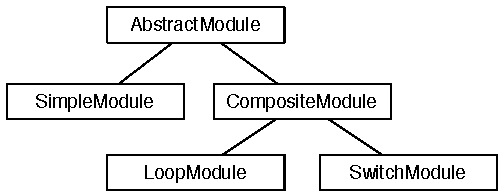
\includegraphics{workflows/module-hierarchy}
	\caption{Module Hierarchy\label{fig:ModuleHierarchy}}
\end{figure}

The hierarchy of modules is also shown in Figure~\ref{fig:ModuleHierarchy}. It is helpful to draw analogies to programming languages:
%
\begin{itemize}
	\item A composite module is a grouping construct for easy reuse of workflows (similar to a block or a function)
	\item A switch module allows the conditional execution of different sub-workflows (similar to a switch/case block)
	\item A loop is the analogue to a repeat-until loop where execution of an iteration (typically) depends on the previous iterations
\end{itemize}

\paragraph{Composite Module}

All composite modules have in- and out-ports just like simple modules. In-ports of a composite module correspond to the formal parameters of a function.

\begin{figure}
	\centering
	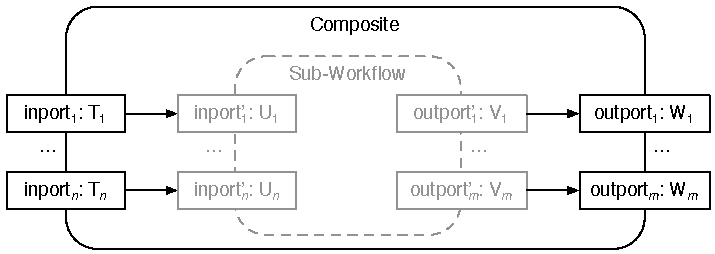
\includegraphics{workflows/composite-module}
	\caption{Composite module. The sub-workflow can be arbitrarily complex.\label{fig:CompositeModule}}
\end{figure}

\paragraph{Switch Modules}

A switch module has a trivial subgraph that consists only of isolated nodes. It has two predefined in-ports: \text{cases} of type \texttt{T[]} and \texttt{value} of type \texttt{T}. On execution, the scheduler will determine the index of \texttt{value} in \texttt{cases}, and then only execute the node in the subgraph with this ID.

\begin{figure}
	\centering
	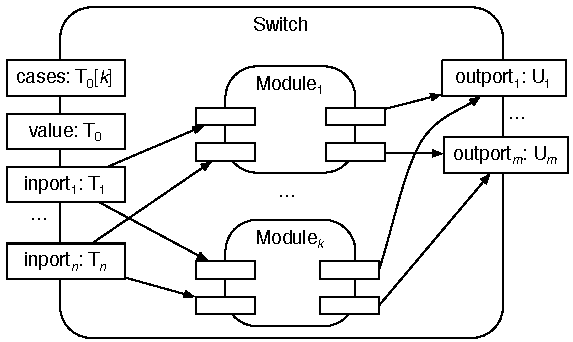
\includegraphics{workflows/switch-module}
	\caption{Switch module. The internal modules may be of arbitrary kind.\label{fig:SwitchModule}}
\end{figure}

\paragraph{Loop Modules}

A loop module has an arbitrary subgraph. Moreover it has a predefined out-port \texttt{continue} of type \texttt{boolean} that determines, after each execution of the sub-workflow, whether the loop module's sub-workflow shoud be executed again. A loop module may have ports that serve both as in\nobreakdash- and out-ports (shown as ``ioports'' in Figure~\ref{fig:LoopModule}). This effectively allows to connect an out-port of the sub-workflow with an in-port of the sub-workflow, in order to pass a value from one iteration to the next.

\begin{figure}
	\centering
	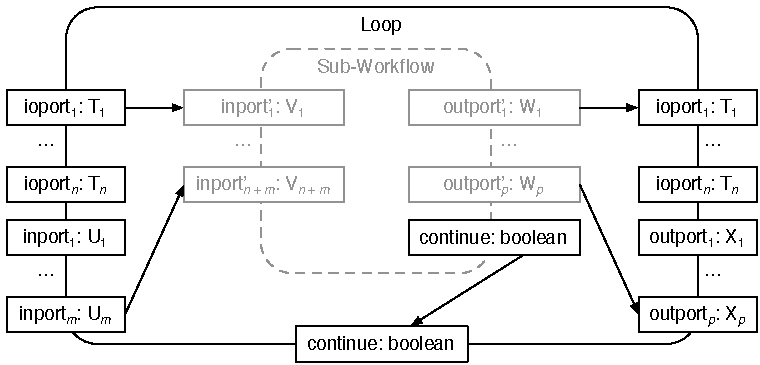
\includegraphics{workflows/loop-module}
	\caption{Loop module. The continue-port is an internal port.\label{fig:LoopModule}}
\end{figure}

\subsection{Data-parallel Module Instances}

Module instances (independent of the module type described before) may be \emph{data-parallel} modules. This property is inferred from the connections a module has in a workflow, as described in the following.

A \emph{split connection} connects an out-port of type \texttt{T[]} to an in-port of type \texttt{U}. Let M denote the module that contains the in-port. A split connection requires that:
%
\begin{itemize}
	\item type \texttt U is type-compatible with type \texttt T,
	\item no other in-port of M has data-parallel connections,
	\item all out-ports of M are connected via a merge connection, i.e., from type \texttt V to type \texttt{W[]}, where \texttt W is type-compatible with type \texttt V.
\end{itemize}
%
A module with split/merge connections is executed using data parallelism, i.e., the module is executed in parallel for each array element of the out-port of the split connection. As part of the merge connection, all out-ports of the module are aggregated into parallel arrays.

\begin{figure}
	\centering
	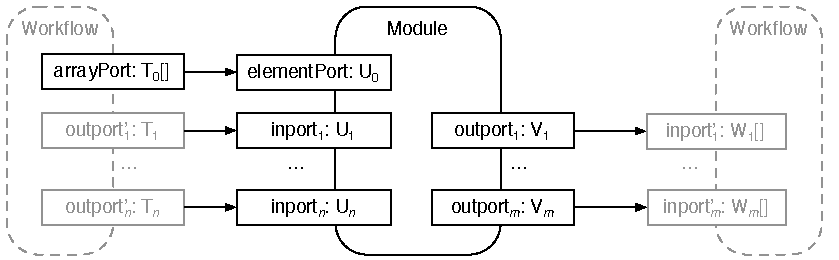
\includegraphics{workflows/data-parallel-module}
	\caption{Data-Parallel module, which may be of arbitrary kind.\label{fig:DataParallelModule}}
\end{figure}

\section{Class Structure} \label{sec:Workflow:ClassStructure}

Workflows are represented by \symlabel{AbstractModule}{sym:AbstractModule} objects. Since the representation contains circular references, these classes are only what is commonly referred to as ``popsicle immutable'': Objects remain mutable until they are explicitly ``frozen''. 
The class structure is shown in Figure~\ref{fig:WorkflowClasses}.

\begin{figure}
\tikzumlset{font=\ttfamily\small}
\centering
\begin{tikzpicture}
	\umlclass[x=10,y=12]{Port}{%
		+ name: String\\
		+ type: Type\\
		+ dimensions: integer
	}{%
		+ freeze()
	}

	\umlclass[x=3,y=12]{AbstractModule}{%
	}{%
		+ freeze()
	}
	
	\umlclass[x=0,y=7]{SimpleModule}{%
	}{%
	}
	\umlinherit[geometry=|-]{SimpleModule}{AbstractModule}
	
	\umlclass[x=6,y=7]{CompositeModule}{%
	}{%
	}
	\umlinherit[geometry=|-, anchor1=70]{CompositeModule}{AbstractModule}

	\umlclass[x=3,y=4]{SwitchModule}{%
	}{%
	}
	\umlinherit{SwitchModule}{CompositeModule}

	\umlclass[x=9,y=4]{LoopModule}{%
	}{%
	}
	\umlinherit{LoopModule}{CompositeModule}
	
	\umluniassoc[geometry=|-|,arg={+ inPorts}, pos=0.9, mult=*, anchor1=90, anchor2=90, arm1=3]{AbstractModule}{Port}
	\umluniaggreg[arg={+ outPorts}, pos=0.3, mult=*, anchor1=-20, anchor2=-152]{AbstractModule}{Port}
	\umluniaggreg[arg={+ inConnections}, mult=*, pos=0.6, angle1=130, angle2=140, loopsize=3cm]{Port}{Port}
	\umluniaggreg[arg={+ outConnections}, mult=*, pos=0.6, angle1=50, angle2=40, loopsize=3cm]{Port}{Port}
	\umluniassoc[arg={+ module}, pos=0.8, mult=1, anchor1=150, anchor2=30]{Port}{AbstractModule}
	\umluniassoc[arg={+ parent}, pos=0.8, mult=0..1, anchor1=-30, anchor2=153]{AbstractModule}{CompositeModule}
	\umluniassoc[geometry=-|, arg={+ modules}, pos=1.8, mult=1..*, anchor1=160, anchor2=-90]{CompositeModule}{AbstractModule}
	\umluniassoc[arg={+ continuePort}, pos=0.9, mult=1]{LoopModule}{Port}
	\umluniassoc[geometry=|-|, arg={+ casePort}, pos=0.6, mult=1, anchor1=-45, anchor2=-65, arm1=-1cm]{SwitchModule}{Port}
	\umluniassoc[geometry=|-|, arg={+ valuePort}, pos=0.8, mult=1, anchor1=-75, anchor2=-45, arm1=-2cm]{SwitchModule}{Port}
\end{tikzpicture}
\caption{Workflow classes.\label{fig:WorkflowClasses}}
\end{figure}

% When using TeXShop on the Mac, let it know the root document. The following must be one of the first 20 lines.
% !TEX root = ../design.tex

\chapter{CloudKeeper Extensibility}

% Abstract. What is the problem we want to solve?
CloudKeeper has a layered, modular architecture that allows user-defined module definitions, languages, and types, without any modifications to the CloudKeeper core.

\section{Requirements}

\subsection{Non-functional}

\begin{enumerate}
	\item \label{enum:NFR:P1} Extensibility: Allow users to extend CloudKeeper according to user needs, without having to ask CloudKeeper developers for support.
	\item \label{enum:NFR:P2} Usability: Extending CloudKeeper with user-defined modules, languages, or types should be easy (e.g., drag-and-drop-like solutions are preferable to editing configuration files).
	\item \label{enum:NFR:P3} Deployment: Easy (no downtime) deployment of functionality across different machines
	\item \label{enum:NFR:P4} Maintainability: Ease of development
\end{enumerate}

\subsection{Functional}

\begin{itemize}
	\item A repository of user-defined modules, languages, and types

		Reason: \ref{enum:NFR:P3}: Plug-Ins should be stored in a central location that is easily accessible to users.

	\item Embedding workflows in other workflows

		Reason: NFR \ref{enum:NFR:P1}, \ref{enum:NFR:P2}: The easiest way to implement new module definitions should be implementing it as a CloudKeeper workflow.

	\item Hot-swapping of plug-ins, i.e., add/remove plug-ins while the CloudKeeper environment is running

		Reason: NFR \ref{enum:NFR:P3}
\end{itemize}

\section{Module Definitions, Languages, and Types as Plug-Ins}

CloudKeeper is (will evolve into) a simple data-flow programming language, with which users develop workflows that link together modules implemented in arbitrary other programming languages (including CloudKeeper itself). As such, CloudKeeper by design is a universal tool for building new tools, and easy extensibility is a core requirement. There are many examples for similar requirements in other products: For instance, higher-level programming languages like Perl, Python, Java, etc.\ all support extensions written in C. Likewise, database systems such as PostgreSQL support user-defined functions, types, and languages as well.

In CloudKeeper, all module definitions, languages, and types are implemented as plug-ins. This gives the advantages of a modular and lean architecture with well-defined interfaces and a clear separation of concerns. All plug-ins have the following properties:
%
\begin{enumerate}
	\item Name: Each plug-in has a name, which follows the reverse-domain-name notation (like Java classes). It is advisable (but not enforced) that different types of plug-ins are kept in different namespaces. E.g., standard CloudKeeper modules reside in the namespace \texttt{com.svbio.cloudkeeper.modules}, whereas language definitions are kept in \texttt{com.svbio.cloudkeeper.languages}.

	\item Macros: Each plug-in can provide a macro generator that will be invoked before the execution phase. These macros can be used in the configuration of other plugins, or from the module code itself. As an example, a bash language plugin may define the macro \texttt{language.bash.exe} that contains the path to the bash executable on the current system. The module declaration for a module ``XYZ'' implemented in bash may then define its command-line invocation string as \texttt{"\$\{language.bash.exe\}" "\$\{modules.current.path\}/xyz.sh"}, where \texttt{modules.current.path} is another macro (provided by the CloudKeeper core).
\end{enumerate}

\subsection{Module Declarations}

Declarations of modules differ for simple modules and composite modules: Since a simple module is implemented in an arbitrary language, crucial information about in-ports and out-ports cannot be inferred but needs to be explicitly declared.

\paragraph{Simple-Module Declarations}

A simple module declaration contains everything any plug-in declaration contains, plus:
%
\begin{enumerate}
	\item In-ports: A list of the in-ports that this module expects.
	\item Out-ports: A list of the out-ports that this module provides.
	\item Command: The command line that should be used to invoke this module. This needs to be a single bash command. The execution happens as follows: First, all macros (i.e., substrings of form \texttt{\$\{macro-name\}}) are substituted with their actual values. Then, the actual command line is passed to bash for execution. Typical command lines might look like:
		\begin{itemize}
			\item \texttt{"\$\{language.bash.exe\}" "\$\{modules.current.path\}/xyz.sh"}
			\item \texttt{"\$\{language.java.exe\}" -jar "\$\{modules.current.path\}/xyz.jar" xzy}
		\end{itemize}
	\item Interface version: The interface version this module expects. This includes the low-level interface (e.g., the local directories where a module can expect its input, and where it should write its outputs to) as well as the language API.

		Should future version of CloudKeeper necessitate interface changes, CloudKeeoper can still execute versioned modules by using the appropriate legacy executor and legacy language API.
	\item Deterministic: Does this module return the same result whenever it is called with the same arguments? Modules that access information outside the control of CloudKeeper (e.g., pseudo-random number generators, the Internet, etc.) are \emph{not} deterministic.
\end{enumerate}

\paragraph{Composite Module Declarations}

A composite-module declaration contains everything any plug-in declaration contains, plus:
%
\begin{enumerate}
	\item Definition: A function that instantiates a \texttt{CompositeModule} object using the data structures as described in Section~\ref{sec:Workflow:ClassStructure}. This indirection exists because composite modules may be defined in different ways:
		\begin{itemize}
			\item Programmatically in Java, using the API to build the data structures, as described in Section~\ref{sec:Workflow:ClassStructure}. In this case, the definition is just a ``function pointer'' to the function containing the programmatic workflow definition.
			\item Using a domain-specific language as described in Chapter~\ref{ch:DSL}. In this case, the definition is the CloudKeeper function that translates the DSL code into the internal workflow representation.
		\end{itemize}
\end{enumerate}

\subsection{Language}

A language declaration currently contains only whatever a plugin declaration contains. In the future, language declarations may provide additional information. Possible options:
\begin{itemize}
	\item Whether a language is considered ``secure'' (execution can be sandboxed) or ``insecure'' (execution may theoretically bring down the whole machine)
	\item A validator that checks whether a module may properly execute (e.g., it may perform syntactical correctness checks of scripts during workflow definition time, rather than at runtime)
\end{itemize}

\subsection{Persistence of Plug-Ins}

Plug-Ins can be added and removed while CloudKeeper is running. For ease of deployment, CloudKeeper plug-ins are stored in the CloudKeeper distributed file store, under the \texttt{/system} hierarchy (see Chapter~\ref{ch:FileStore}). The default replication level for each file under in this directory is ``everywhere''.
Plug-ins are declared using JSON configuration files.

\begin{example}
Suppose we implement a module \texttt{com.svbio.cloudkeeper.modules.sum} in bash that sums up two integers. It consists of the following two files under \\\texttt{/system/com/svbio/cloudkeeper/modules/sum}:
\begin{itemize}
	\item \texttt{Info.json}: The module declaration. It might look as follows:
		\begin{lstlisting}[gobble=12]
			{
			   "type": "com.svbio.cloudkeeper.metadata.SimpleModuleDeclaration"
			   "name": "com.svbio.cloudkeeper.modules.sum",
			   "command": "${language.bash.exe}" ${modules.current.path}/sum.sh",
			   "inports": [ {
			           "name": "Num1",
			           "elementtype": "com.svbio.cloudkeeper.types.integer",
			           "dimension": 0
			       }, {
			           "name": "Num2",
			           "elementtype": "com.svbio.cloudkeeper.types.integer",
			           "dimension": 0
			       }
			   ],
			   "outports": [ {
			           "name": "Sum",
			           "elementtype": "com.svbio.cloudkeeper.types.integer",
			           "dimension": 0
			       }
			   ],
			   "deterministic": true
			}
		\end{lstlisting}
	\item \texttt{sum.sh}: The bash script that does the actual work. It might look as follows:
		\begin{lstlisting}[gobble=12]
			#!/bin/bash
			NUM1=$(getInput Num1)
			NUM2=$(getInput Num2)
			RESULT=$(echo "$NUM1 + $NUM2" | bc)
			setOutput Sum "$RESULT"
		\end{lstlisting}
\end{itemize}
Of course, languages and types (e.g., \texttt{com.svbio.cloudkeeper.types.integer}) are declared correspondingly.
\end{example}

\subsection{Class Structure}

Plugin declarations are represented by \texttt{PluginDefinition} objects. The class structure is shown in Figure~\ref{fig:PlugIns:Classes}.

Moreover, there is a \texttt{Repository} interface for loading plug-ins from persistent storage into \texttt{PluginDefinition} objects (see Figure~\ref{fig:PlugIns:RepositoryClasses}). An implementation complying with the previous section would scan the \texttt{/system} hierarchy in the file store, parse the \texttt{Info.json} files, and then instantiate the in-memory objects accordingly. For testing and during development, mock \texttt{Repository} objects can be used that generate \texttt{PluginDefinition} objects on-the-fly. When referring to plugins, it is generally cumbersomes having to deal with long names like \texttt{com.svbio.cloudkeeper.modules.sum}. Instead, it is convenient to have the notion of a current namespace and a set of imported names (like, e.g., in Java, where the current namespace is the package where the current class is defined, and names can be imported using the \texttt{import} statement). The equivalent in CloudKeeper is represented by the \texttt{Context} interface. A \texttt{Context} an be created from a \texttt{Repository} using the \texttt{createContextBuilder()} method, which sets the current namespace. Afterwards, the \texttt{addImport()} method may be used on the \texttt{ContextBuilder} object to bring other names into the current scope (context).

\begin{figure}
\tikzumlset{font=\ttfamily\small}
\centering
\begin{tikzpicture}
	\umlclass[x=0,y=6]{PortDefinition}{%
		+ name: String
	}{%
	}

	\umlclass[x=0,y=3,type=interface]{PortType}{%
		+ elementType: Class<?> \\
		+ dimensions: int
	}{%
	}

	\umlclass[x=6,y=15,type=interface]{PluginDefinition}{%
	}{%
		+ getName(): String\\
		+ getMacros(): Map<String, String>
	}

	\umlclass[x=3,y=12]{AbstractModuleDefinition}{%
		+ name: String
	}{%
		+ newInstance(name: String): AbstractModule
	}
	\umlinherit{AbstractModuleDefinition}{PluginDefinition}

	\umlclass[x=10,y=12]{LanguageDefinition}{%
	}{%
	}
	\umlinherit{LanguageDefinition}{PluginDefinition}

	\umlclass[x=0,y=9]{SimpleModuleDefinition}{%
		+ interfaceVersion: int \\
		+ command: String \\

	}{%
	}
	\umlinherit{SimpleModuleDefinition}{AbstractModuleDefinition}

	\umlclass[x=6,y=9]{CompositeModuleDefinition}{%
		+ definition:\\
		  (CompositeModule -> void)
	}{%
	}
	\umlinherit{CompositeModuleDefinition}{AbstractModuleDefinition}

	\umluniassoc[arg={+ type}]{PortDefinition}{PortType}
	\umluniaggreg[arg={+ inPorts}, mult=*, pos=0.5, anchor1=-140, anchor2=150]{SimpleModuleDefinition}{PortDefinition}
	\umluniaggreg[arg={+ outPorts}, mult=*, pos=0.5, anchor1=-40, anchor2=30]{SimpleModuleDefinition}{PortDefinition}
\end{tikzpicture}
\caption{Extensibiliy classes.\label{fig:PlugIns:Classes}}
\end{figure}

\begin{figure}
\tikzumlset{font=\ttfamily\small}
\centering
\begin{tikzpicture}
	\umlclass[x=0,y=0,type=interface]{Repository.ContextBuilder}{%
	}{%
		+ addImport(String name): \\ContextBuilder\\
		+ build(): Context
	}

	\umlclass[x=9,y=5,type=interface]{Context}{%
	}{%
		+ getPlugin(): PluginDefinition\\
		+ getModuleDefinition(): \\AbstractModuleDefinition\\
		+ getLanguageDefinition(): \\LanguageDefinition
	}

	\umlclass[x=9,y=0,type=interface]{Repository}{%
	}{%
		+ createContextBuilder\\(currentNamespace: String): \\ContextBuilder\\
		+ getMacros(): Map<String,String>
	}
	\umlinherit{Repository}{Context}
\end{tikzpicture}
\caption{Repository and Namespace Interfaces.\label{fig:PlugIns:RepositoryClasses}}
\end{figure}

% When using TeXShop on the Mac, let it know the root document. The following must be one of the first 20 lines.
% !TEX root = ../design.tex

\chapter{Type System} \label{sec:TypeSystem}

An out-port is \emph{type-compatible} with an in-port if one of the following criteria holds:
\begin{itemize}
	\item the out-port type and in-port type are the same
	\item there is an implicit conversion rule from the out-port type to the in-port type
	\item one of the previous two conditions holds, and data parallelism can be inferred from the edge.
\end{itemize}

% When using TeXShop on the Mac, let it know the root document. The following must be one of the first 20 lines.
% !TEX root = ../design.tex

\chapter{Workflow Langauge} \label{ch:DSL}

% Abstract. What is the problem we want to solve?
CloudKeeper is a simple data-flow programming language, with which users develop workflows that link together modules implemented in arbitrary other programming languages (including CloudKeeper itself). This language has a very simple grammar, is therefore easy to learn, is statically typed, has full type inference, and bears resemblance to modern programming languages like Scala and Java.

\section{Requirements}

\subsection{Non-functional}

\begin{enumerate}
	\item \label{enum:NFR:D1} Usability: Ease of use
\end{enumerate}

\subsection{Functional}

\begin{itemize}
	\item Allow easy conversion between a graphical representation and code
		
		Reason: NFR \ref{enum:NFR:D1}
\end{itemize}

\section{Domain-Specific Language}

It is most instructive to start with an example. The workflow shown in Figure~\ref{fig:WorkflowExample} could defined using the CloudKeeper language as follows:

\begin{lstlisting}
package com.svbio.cloudkeeper.modules;

def logRegr = (path) -> {
    initialLL = "-infinity"
    initialZeroVector = null
    loop = loop((path = path, coef = initialZeroVector, loglikelihood = initialLL) -> {
        splitInput = split_input(path)
        logRegrStep = log_regr_step(file = splitInput.files, coef = coef)
        sumXtX = sum(logRegrStep.XtX)
        invertXtX = invert_matrix(sumXtX)
        sumXty = sum(logRegrStep.Xty)
        newCoef = prod([invertXtX, sumXty])
        sumLL = sum(logRegrStep.loglikelihood)
        checkLL = check_ll(oldLL = loglikelihood, newLL = sumLL)
        return (continue = checkLL.continue, coef = newCoef, loglikelihood = sumLL)
    })
    return (coef = loop.coef)
}
\end{lstlisting}

Crucial properties of the language are:
\begin{itemize}
	\item Support for both named arguments and named return values.
	\item Workflows are first-class values (even though in the first implementation, they may only be used in for, switch, and loop blocks).
	\item Execution order is independent of the statement order, and is only dependent on the directed graph defined by the statements. However, for simplicity, names need to be defined before they can be used, i.e., not every permutation of the statements within a block is a valid program. (This constraint is possible because workflows graphs are acyclic.)
\end{itemize}

Line 14 could be replaced by native CloudKeeper code:
\begin{lstlisting}
        checkLL = switch(value = abs(sumLL - loglikelihood) < 0.001, {
            "true": { return (continue = true) },
            "false": { return (continue = false) }
        })
\end{lstlisting}
Here, the second argument to \texttt{switch} is a dictionary (which uses the same notation as in Python).

% When using TeXShop on the Mac, let it know the root document. The following must be one of the first 20 lines.
% !TEX root = ../design.tex

\chapter{Interpreter} \label{ch:interpreter}

% Abstract. What is the problem we want to solve?
The description has been moved out of the design document to a stand-alone paper (see \texttt{paper.tex}).

\printbibliography

\end{document}
